\documentclass[a4paper]{article}
\usepackage{color}
\usepackage{tikz}
\usepackage{lipsum}
\usepackage{geometry}
\geometry{a4paper, left=3cm, top=3cm, bottom=3cm, right=3cm}
\usepackage{changepage}
\usepackage{booktabs}
\usepackage[labelfont = sc]{caption}
\DeclareCaptionFormat{mycaptionfont}{\fontsize{12}{13}\selectfont#1#2#3}
\usepackage{threeparttable}
\usepackage{graphicx}
\usepackage{ntheorem}
\usepackage{caption}
\captionsetup{format=mycaptionfont}
\usepackage{subcaption}
\theoremseparator{:}
\newtheorem{hyp}{Hypothesis}
\usetikzlibrary{shapes,decorations,arrows,calc,arrows.meta,fit,positioning}
\tikzset{
    -Latex,auto,node distance =1 cm and 1 cm,semithick,
    state/.style ={ellipse, draw, minimum width = 0.7 cm},
    point/.style = {circle, draw, inner sep=0.04cm,fill,node contents={}},
    bidirected/.style={Latex-Latex,dashed},
    el/.style = {inner sep=2pt, align=left, sloped}
}





\begin{document}
\section{Data Prep, EDA, and Theory development}
\subsection{Varaible Selection \& Explanation}
For the purpoase of analyzing the determinants of prices of home sales in the US, the followign variables were included in the analysis (Table 1): 


\begin{itemize}
  \item Sale Price (DV)
  \item Total Living Space (IV) \& Years Since Remodeling (at point of Sale) (IV)
  \item Confounders \& Controls: Quality, Lot Area, Condition
\end{itemize}


As can be seen in Table 1, a total of 1,460 house sales were recorded between 2006 and 2010 for the district of Ames, Iowa (USA). The dependent varibale was identified to be SalePrice. As can be observed in Table 1, the mean sale price of a house was (in 1000s) \$180.921 (SD = 79.443). Combined with the range [34,900, 755,000] a positive skewness was to be expected (skew = 1.881), considering that the outcome variable is a of financial nature. The Total Living Area displays a mean of 2,572.89 square feet (SD = 823.598) in addition to a large range of values[334, 11,752].  
Years Since remodeling (at time of sale) shows that the average property did not undergo renovations for 22.95 (~23) years (SD = 20.950). Contrary to expectation, this varaible distributes reasonably equally across the range, stopping out at a maximum of 60 years (See Figure 1B - quantiles).
Furhermore, the variable Quality (and Condition) represents a rating from 1 to 10, similar to a Likert Scale. Quality has to be considered a categorical variable in this case i.a. because the distances between each rating level are not constant and the distribution is skewed \textbf{(SEE SUPPLEMENTARY APPENDIX REGRESSION AND PICTURE)}. However, while strictrly speakign there we cannot consider Quality a numerical variable, for the purpose of certain examples at a later point, this variable will be considered as both a categorical and numerical variable (no inference will be made is used as numerical). Finally, Lot Area, will be used as a confounder in the regressions to control for the association larger lot sizes creating larger houses (\textbf{AS AN INTERACTION}). 


% Table created by stargazer v.5.2.3 by Marek Hlavac, Social Policy Institute. E-mail: marek.hlavac at gmail.com
% Date and time: Wed, Sep 14, 2022 - 15:53:27
\begin{table}[!htbp] 
\begin{adjustwidth}{-0.5cm}{-0cm}
\begin{threeparttable}
\small
\captionsetup{font=small, justification=raggedright,singlelinecheck=false}
\caption{\textsc{Descriptive Statistics of Numeric Varaibles}}
\centering 
  \label{}   
\begin{tabular}{@{\extracolsep{5pt}}lccccccc} 
\\[-5ex]\hline 
\hline \\[-1.8ex] 
Statistic & \multicolumn{1}{c}{Mean} & \multicolumn{1}{c}{St. Dev.} & \multicolumn{1}{c}{Min} & \multicolumn{1}{c}{Pctl(25)} & \multicolumn{1}{c}{Median} & \multicolumn{1}{c}{Pctl(75)} & \multicolumn{1}{c}{Max} \\ 
\hline \\[-1.8ex] 
SalePrice & 180.921 & 79.443 & 34.900 & 129.975 & 163.000 & 214.000 & 755.000 \\ 
Lot Area & 10,516.830 & 9,981.265 & 1,300 & 7,553.5 & 9,478.5 & 11,601.5 & 215,245 \\ 
Quality & 6.099 & 1.383 & 1 & 5 & 6 & 7 & 10 \\ 
Condition & 5.575 & 1.113 & 1 & 5 & 5 & 6 & 9 \\ 
Total Living Space & 2,572.893 & 823.598 & 334 & 2,014 & 2,479 & 3,008.5 & 11,752 \\ 
Years Since Remodeling & 22.950 & 20.641 & 0 & 4 & 14 & 41 & 60 \\ 
\hline \\[-3.5ex] 
\end{tabular} 
\begin{tablenotes}[para,flushleft]
      \small
      \item\textit{Notes:} N = 1460. OLS estimates, robust standard errors in parentheses.*** p$<$0.01, ** p$<$0.05, * p$<$0.1
    \end{tablenotes}
\end{threeparttable}
\end{adjustwidth}
\end{table}


Beyond this table, there are multiple categorical variables \textbf{(see Appendix)}, such as Zoning and Year of Sale. The original (MS)Zoning variable contains seven categories, of which five contain data; these zones correspond to the administrative classification of the ground on which the properties are constructed (Commercial, Floating Village, Low-Density, Moderate-Density, High-Density contain data; Residential Low Density Park, Agriculutural, Industrial do not contain records). For the purpose of this analysis, this number was reduced to four categories based on the similar behaviour of Moderate and High Density properties \textbf{(SEE SUPLEMENTARY APPENDIX PLOT)} in  the data as Ames, Iowa, represents the steretypical picture of a mid-western town in the US, thereby displaying fewer densly populated areas. Thus, the main question of this analysis section focuses on the difference between Low and higher density properties.\footnote{Floating Village and Commercial behave too differently to be merged} In addition, year of sale will be used to control for the effect of the 2008/2009 housing cricis. 






% FIGURE 
\begin{figure}
     \centering
     \begin{subfigure}[b]{0.45\textwidth}
         \centering
         \includegraphics[scale=0.3]{"/home/angelo/Documents/Uni/Courses/Advanced Statistics and programming/Assignments/assignment1/Code/h1.jpg"}
         \caption{Positive association of total Living Space \& Sale Price \& optimal line}
         \label{fig:y equals x}
     \end{subfigure}
     \hfill
     \begin{subfigure}[b]{0.45\textwidth}
         \centering
         \includegraphics[scale=0.30]{"/home/angelo/Documents/Uni/Courses/Advanced Statistics and programming/Assignments/assignment1/Code/h3.jpg"}
         \caption{Positive association of total Living Space \& Sale Price}
         \label{fig:three sin x}
     \end{subfigure}
     \hfill
     \begin{subfigure}[b]{0.45\textwidth}
         \centering
         \includegraphics[scale=0.325]{"/home/angelo/Documents/Uni/Courses/Advanced Statistics and programming/Assignments/assignment1/Code/h2.2.jpg"}
         \caption{Positive association of total Living Space \& Sale Price}
         \label{fig:five over x}
     \end{subfigure}
        \caption{Three Hypothesis Graphs displaying their repective association with the outcome variable}
        \label{fig:three graphs}
\end{figure}


Finally, the plots are to be considered in the context of the hypothesis in the next section. 


















\begin{center}
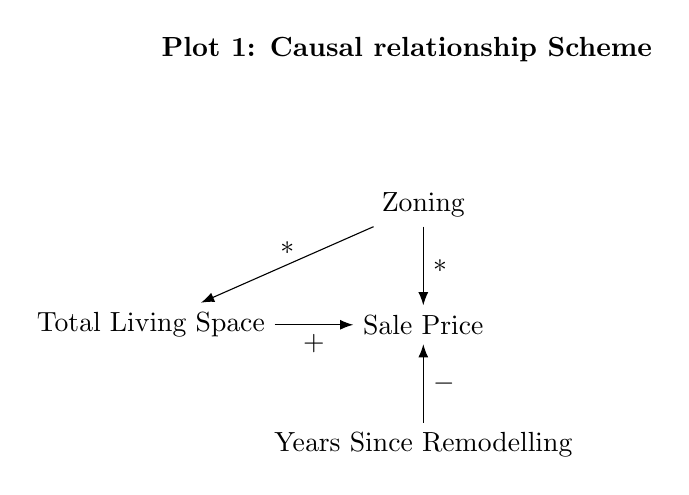
\begin{tikzpicture}
	\centering
 	\node at (3.25,3.5) {\textbf{Plot 1: Causal relationship Scheme}};
    \node (1) at (0,0) {Total Living Space};
	\node (2) [right = of 1] {Sale Price};
	\node (3) [above = of 2] {Zoning};
	\node (4) [below = of 2] {Years Since Remodelling};

	\path (1) edge node[below] {$+$} (2);
	\path (3) edge node[right] {$*$} (2);
	\path (3) edge node[above] {$*$} (1);
	\path (4) edge node[right] {$-$} (2);
	
\end{tikzpicture}
\end{center}




\end{document}
